\documentclass{beamer}
\usetheme{CambridgeUs}  
\usepackage[]{graphicx}
\usepackage{caption}
\usepackage{subcaption}
\usepackage{media9}
\usepackage{cite}


\title{Hall's Theorem}
\author{Himanshu Prajapati}
\institute{Indian Institute of Technology, Guwahati}
\date{\today}
\logo{
\includegraphics[height=1cm]{logo.png}}

\begin{document}
	
	\begin{frame}
		
		\titlepage
		
	\end{frame}
	
	\section{Outline}
	\begin{frame}{Outline}
		
		\begin{itemize}
			\item Bipartite Graph
			\item Matching
			\item Hall's Theorem
			\item Proof
			\item Corollary
			
			
		\end{itemize}
		
	\end{frame}
	
	\section{Bipartite Graph}
	\begin{frame}{Bipartite Graph}
		
		\begin{block}{Definition}
			 A graph is bipartite if its vertex set can be partitioned into two nonempty subsets $X$ and $Y$ such that each edge of $G$ has one end in $X$ and the other in $Y$. The pair $(X, Y)$ is called a bipartition of the bipartite graph. The bipartite graph $G$ with bipartition $(X, Y)$ is denoted by $G[X, Y]$.
		\end{block}
		
	\end{frame}

	\section{Bipartite Graph}
	\begin{frame}{Example}
		
	     \begin{figure}
	     	\centering
	     	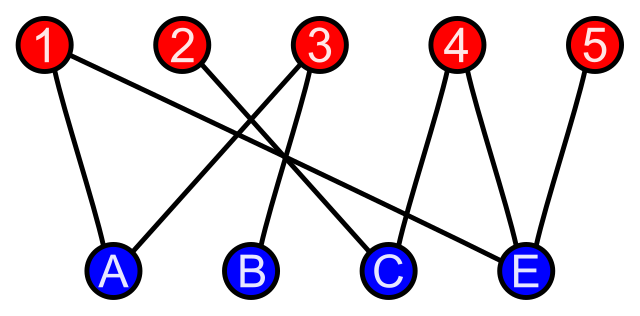
\includegraphics[height=4cm,width=10cm]{Bipartite_fig.png}
	     	\caption{Example of Bipartite Graph}
	     	\label{fig1}
	     \end{figure}
		
	\end{frame}
	\section{Matching}
	\begin{frame}{Matching}
		
		\begin{itemize}
			\item A subset $M$ of the edge set $E$ of a loopless graph $G$ is called independent if no two edges of $M$ are adjacent in $G$.
			
			\item  A matching in $G$ is a set of independent edges.
			
			\item A set $S$ of vertices of $G$ is said to be saturated by a matching $M$ of $G$ or $M$-saturated if every vertex of $S$ is incident to some edge of $M$. A vertex $v$ of $G$ is $M$-saturated if $fv$ is $M$-saturated. $v$ is $M$-unsaturated if it is not $M$-saturated.
		\end{itemize}
		
	\end{frame}
	
	\begin{frame}{Definition}
		
			Let $G$ be a bipartite graph on the parts $X$ and $Y$, and let $S$ be a matching of $G$. If every vertex in $X$ is covered by an edge of $S$, then we say that $S$ 
			is a perfect matching of $X$ into $Y$.
			
			For a graph $G$ and a subset $T$ of $V(G)$, we let $N_G(T)$ denote the set of vertices of $G$ that are adjacent to some vertex in $T$, that is,
			\[
			N_G(T) := \{v \in V(G) \,|\, vw \in E(G) \text{ for some } w \in T\}.
			\]
			
			Observe that if $G$ is bipartite on the parts $A$ and $B$, then $N_G(T) \subseteq B$ for any $T \subseteq A$.
		
	\end{frame}
	
	\section{Hall's Theorem}
	\begin{frame}{Hall's Theorem}
		
			
			\begin{block}{Statement}
			     	\textit{For a bipartite graph $G$ on the parts $X$ and $Y$, the following conditions are equivalent.
			     	\begin{enumerate}
			     		\item[(a)] There is a perfect matching of $X$ into $Y$.
			     		\item[(b)] For each $T \subseteq X$, the inequality $|T| \leq |N_G(T)|$ holds.
			     \end{enumerate}}
			\end{block}
	\end{frame}

	
     \section{Proof}
     \begin{frame}{Proof}
     
     		(a) $\Rightarrow$ (b): \\
     		Let $S$ be a perfect matching of $X$ into $Y$. As $S$ is a perfect matching, for every $x \in X$, there exists a unique $y_x \in Y$ such that $xy_x \in S$. Define the map $f : X \to Y$ by $f(x) = y_x$. Since $S$ is a matching, the function $f$ is injective. Therefore, for any $T \subseteq X$, we see that $|T| = |f(T)| \leq |N_G(T)|$ because $f(T) \subseteq N_G(T)$ .
      \end{frame}
	
	\begin{frame}{Proof(continued)}
			(b) $\Rightarrow$ (a):\\
			 Conversely, suppose that $|T| \leq |N_G(T)|$ for each $T \subseteq X$. We will prove that there exists a perfect matching of $X$ into $Y$ by induction on $n := |X|$. If $n = 1$, then the only vertex $x$ in $X$ must be adjacent to some vertex $y$ in $Y$ by condition (b), and, therefore, $\{xy\}$ is a perfect matching of $X$ into $Y$. Now assume that every bipartite graph on the parts $X_0$ and $Y_0$ with $|X_0| < |X|$ and satisfying condition (b) has a perfect matching of $X_0$ into $Y_0$. We split the rest of the proof into two cases.
		
	\end{frame}

   \begin{frame}{Proof(continued)}
   	 	\textbf{Case 1:} For every nonempty proper subset $T$ of $X$ (that is, $T \subset X$), the strict inequality $|T| < |N_G(T)|$ holds. Take $x \in X$ and $y \in $NG($\{x\}$). Let $G_0$ be the bipartite graph we obtain by removing $x$ and $y$ (and the edges incident to them) from $G$. Now for every subset $A$ of $X \setminus \{x\}$, we see that
   	 \[
   	 |N_{G_0}(A)| \geq |N_G(A)| - 1 \geq |A|,
   	 \]
   	 where the last inequality holds because $A$ is a strict subset of $X$. By induction hypothesis, there exists a perfect matching $S_0$ in $G_0$ of $X \setminus \{x\}$ into $Y \setminus \{y\}$. It is clear now that $S_0 \cup \{xy\}$ is a perfect matching in $G$ of $X$ into $Y$.
   \end{frame}

   \begin{frame}{Proof(continued)}
   	  	\textbf{Case 2:} There exists a nonempty proper subset $A$ of $X$ such that $|A| = |N_G(A)|$. Let $G_1$ be the subgraph of $G$ induced by the set of vertices $A \cup N_G(A)$, and let $G_2$ be the subgraph of $G$ we obtain by removing $A \cup N_G(A)$ (and their incident edges) from $G$. It is clear that $G_1 = (A, N_G(A))$ and $G_2 = (X \setminus A, Y \setminus N_G(A))$ are bipartite graphs.
   	  
   	  Let us show that both $G_1$ and $G_2$ satisfy condition (b). To show that $G_1$ satisfies (b), take $T \subseteq A$. It follows by the way $G_1$ was constructed that $N_{G_1}(T) = N_G(T)$. As a result, $|N_{G_1}(T)| = |N_G(T)| \geq |T|$. Then $G_1$ satisfies condition (b). In order to argue that $G_2$ also satisfies condition (b), take $T_0 \subseteq X \setminus A$ and observe that $N_{G_2}(T_0 \cup A) = N_G(A) \cup N_{G_2}(T_0)$, where the union on the right-hand side is disjoint. Since $|N_{G_2}(T_0 \cup A)| \geq |T_0 \cup A|$ and $|N_G(A)| = |A|$, $|N_{G_2}(T_0)| = |N_{G_2}(T_0 \cup A)| - |N_{G_1}(A)| \geq |T_0 \cup A| - |A| = (|T_0| + |A|) - |A| = |T_0|$. Therefore, $G_2$ also satisfies condition (b).
   \end{frame}
    
    \begin{frame}{Proof(Continued)}
    	Since $|A| < |X|$ and $|X \setminus A| < |X|$, our induction hypothesis guarantees the existence of a perfect matching $S_1$ in $G_1$ of $A$ into $N_G(A)$ and a perfect matching $S_2$ in $G_2$ of $X \setminus A$ into $Y \setminus N_G(A)$. Then it follows from the construction of $G_1$ and $G_2$ that $S_1 \cup S_2$ is a perfect matching in $G$ of $X$ into $Y$, which concludes the proof.
    \end{frame}

	\section{Corollary}
	\begin{frame}{Corollary}
		\begin{block}{Statement}
			\textit{A $k(>1)$-regular bipartite graph is 1-factorable}
		\end{block}
		
	\end{frame}
     
     \begin{frame}{Proof}
     	Let $G$ be a $k$-regular bipartite graph with bipartition $X$ and $Y$. Then, $E(G)$ is the set of edges incident to the vertices of $X$ and is also equal to the set of edges incident to the vertices of $Y$. Hence, $k|X| = |E(G)| = k|Y|$, and therefore $|X| = |Y|$. 
     	
     	Now, consider any subset $S \subseteq X$. By the definition of a bipartite graph, the neighborhood of $S$, denoted as $N(S)$, is contained in $Y$, and $N(N(S))$ contains $S$. 
     	
     	Let $E_1$ and $E_2$ be the sets of edges of $G$ incident to $S$ and $N(S)$, respectively. Then, $E_1 \cup E_2$ contains all the edges of $G$ incident to vertices in $S$. We have $|E_1| = k|S|$ and $|E_2| = k|N(S)|$. Therefore, since $|E_1| + |E_2| = |E_1 \cup E_2| \leq k|S|$, it follows that $k|N(S)| \leq k|S|$. 
     	
     	As $k > 1$, we can conclude that $|N(S)| \leq |S|$. 
     \end{frame}
 
    \begin{frame}{Proof(Continued)}
    	So, by Hall's theorem, $G$ has a matching that saturates all the vertices of $X$, which means that $G$ has a perfect matching $M$. 
    	
    	Deletion of the edges in $M$ from $G$ results in a $(k - 1)$-regular bipartite graph. 
    	
    	Repeated application of this argument shows that $G$ is 1-factorable.
    \end{frame}
	
	\section{References}
	\begin{frame}{References}
	%	\cite{example ,another}
		\bibliographystyle{unsrt}
		\bibliography{refrence}
	\end{frame}
	
	\begin{frame}
		\centering
		\Huge{Thank You}
	\end{frame}
	
	
	
\end{document}

